\documentclass[11pt]{article}
\usepackage{url}
\usepackage{enumerate}
\usepackage{graphicx}
\usepackage{float}
\renewcommand{\thesection}{\Roman{section}} 
\renewcommand{\thesubsection}{\arabic{subsection}}
\title{\textbf{Generation of a 3D object from a Digital Elevation Model (DEM)}}
\author{\textbf{Supervisor: Prof. Pascal Desbarats}\\\\
		VU Manh Tu\\
		NGUYEN Bao Xuan Truong\\
		HO Do Quynh Phuong\\
		PHAM Phu Quoc\\
		BUI The Anh		
		}
\date{06-04-2016}

\begin{document}
\maketitle
\section{Project description}
\subsection{Project overview}
This report outlines the design and development of a computer software to visualize DEM files, which are from different formats, in 3-Dimensions. It allows users using several convenient functionalities such as rotations, translation, zoom along the axises, resizing or cropping using boundary boxes, creating a support at its basis to transform it into 3D object, labeling it on. The result can be exported in OBJ and STL formats. 

The solution should be developed on \emph{C++ / Qt framework}\footnote{\url{http://www.qt.io/ide/}} and a visualisation in \emph{OpenGL}\footnote{Opengl-superbible-comprehensive-tutorial-and-reference-5th-edition-2010}.

\subsection{Concepts}
\subsubsection{What is digital elevation model (DEM)?}
A digital elevation model (DEM) is a digital model or 3D representation of a terrain's surface — commonly for a planet (including Earth), moon, or asteroid — created from terrain elevation data.
\par\noindent It is 2D map in which each point is associated with its height. DEM can be obtained through techniques such as photogrammetry, lidar, land, surveying, etc.\footnote{\url{https://en.wikipedia.org/wiki/Digital_elevation_model}}


\subsubsection{DEM file formats}

\underline{USGS DEM}\\
The USGS DEM format is a standard format for the storage of raster digital elevation data. The USGS has produced five different digital elevation products  with the primary differing characteristic being the spacing, or sampling interval, of the data:\footnote{\url{http://agdc.usgs.gov/data/usgs/geodata/dem/dugdem.pdf}}
\begin{itemize}
\item 7.5-Minute DEM 30- x 30-meter data spacing
\item 2-Arc-Second DEM 2- x 2-arc-second data spacing
\item 15-Minute Alaska DEM 2- x 3-arc-second data spacing
\item 7.5-Minute Alaska DEM 1- x 2-arc-second data spacing
\item 1-degree DEM 3- x 3-arc-second data spacing
\end{itemize}

\noindent\textit{Purpose} 
\\ DEM file is used in the generation of three-dimensional graphics displaying terrain slope, aspect (direction of slope), and terrain profiles between selected points. At the USGS, DEMs have been used in combination with digital raster graphics (DRG's), digital line graphs (DLG's), and digital orthophoto quadrangles (DOQ's) to both enhance the visual information for data extraction and revision purposes and to create aesthetically pleasing and dramatic hybrid digital images. Non-graphic applications such as modeling terrain and gravity data for use in the search for energy resources, calculating the volume of proposed reservoirs, and determining landslide probability have also been developed.\footnote{\url{http://www.softree.com/Tips_Techniques/T-004-USGS-DEM/USGS_DEM.pdf}}
\\\\ \textit{Structure} 
\\ DEM file is an ASCII file format consisting of a header record (Type A), data records (Type B) and an accuracy metadata record (Type C)\footnote{\url{http://www.geobc.gov.bc.ca/base-mapping/atlas/trim/specs/BC-DEM-specifications-2002-12.pdf}}
\\ The physical structure of the DEM distributed to the user is as follows:\footnotemark[4]
\begin{itemize}
\item Data recorded in fixed-block format on unlabeled or ANSI-labeled 9-track magnetic tape at 1,600 or 6,250 bpi density. 
\item Logical record size of 1,024 bytes. No more than one logical record type (A, B, or C) recorded in any 1,024-byte record. However, more than one 1,024-byte record is usually required to store a single record type B. The logical record is padded with blanks if necessary to fill to the end of the 
logical record. Bytes 1,021-1,024 of each logical record are padded with blanks. 
\item Physical record size of 4,096 bytes; that is, 4 logical records per physical record. 
\item Data written as ANSI-standard ASCII characters.
\end{itemize}

\noindent \underline{SDTS DEM}\\
SDTS stands for Spatial Data Transfer Standard, is a robust way of transferring earth-referenced spatial data between dissimilar computer systems with the potential for no information loss. It is a transfer standard that embraces the philosophy of self-contained transfers, i.e. spatial data attribute, dereferencing, data quality report, data dictionary, and other supporting metadata all included in the transfer. \footnote{\url{http://mcmcweb.er.usgs.gov/sdts/whatsdts.html}}\\ 
SDTS has 7 parts. Parts 1-3 are about SDTS specification which is organized into the base specification, all of them are related, but relatively independent. Parts 4-6 are about multiple profiles, each define specific rules and formats for applying SDTS for the exchange of particular types of data in SDTS: \footnote{\url{http://mcmcweb.er.usgs.gov/sdts/standard.html}}
\begin{itemize}
\item Part 1 – Logical Specifications:
\par\noindent It consists of three main sections, which explain the SDTS conceptual model and SDTS spatial object types, components of a data quality report, and the layout of all SDTS modules.
\item Part 2 – Spatial Features: 
\par\noindent It contains a catalogue of spatial features and associated attributes. This part addresses a need for definition of common spatial feature terms to ensure greater compatibility in data transfers. The current version of Part 2 is limited to small- and medium-scale spatial features commonly used on topographic quadrangle maps and hydrographic charts.
\item Part 3 – ISO 8211 Encoding: 
\par\noindent This part explains the use of a general purpose file exchange standard, ISO 8211, to create SDTS file sets (i.e. transfers).
\item Part 4 - Topological Vector Profile:\\
The Topological Vector Profile (TVP) is the first of a potential series of SDTS profiles, each of which defines how the SDTS base specification (Parts 1, 2, and 3) must be implemented for a particular type of data. The TVP limits options and identifies specific requirements for SDTS transfers of data sets consisting of topologically structured area and linear spatial features.
\item Part 5 - Raster Profile and Extensions: 
\par\noindent The Raster Profile is for 2-dimensional image and gridded raster data. It permits alternate image file formats using the ISO Basic Image Interchange Format (BIIF) or Dereferenced Tagged information File Format (Geo TIFF).
\item Part 6 - Point Profile: 
\par\noindent The Point Profile contains specifications for use with geographic point data only, with the option to carry high precision coordinates such as those required for geodetic network control points. This profile is a modification of Part 4, the Topological Vector Profile, and follows many of the conventions of that profile.
\end{itemize}

\noindent \underline{DTED}\\ 
DTED is a standard of digital datasets which consists of a matrix of terrain elevation values \footnote{\url{https://en.wikipedia.org/wiki/DTED}}. It is the oldest digital mapping format that we still use today. This standard was originally developed in the 1970s by NIMA - the National Imagery and Mapping Agency. DTED was originally developed to drive 3D milling machines and provide elevation data needed for cruise missile planning. \footnote{\url{http://www.mission-planning.com/DTED_Part1.htm}}\\ 
DTED format have 3 level:\footnote{\url{http://fas.org/irp/program/core/dted.htm}}
\begin{itemize}
\item Level 0 
\begin{itemize}
\item Has a post spacing of approximately 900 meters.
\item Elevation post spacing is 30 arc second 
\item Derived from NIMA DTED Level 1 to support a federal agency requirement
\item DTED Level 0 may be of value to scientific, technical, and other communities for and applications that require terrain elevation, slope, and/or surface roughness information. It allows a gross representation of the Earth's surface for general modeling and assessment activities. Such reduced resolution data is not intended and should not be used for automated flight guidance or other precision activity involving the safety of the public.
\end{itemize}
\item Level 1 
\begin{itemize}
\item Has a post spacing of approximately 90 meters.
\item A uniform matrix of terrain elevation values with post spacing every 3 arc seconds
\item The information content is approximately equivalent to the contour information represented on a 250,000 scale map.
\end{itemize}
\item Level 2 
\begin{itemize}
\item Has a post spacing of approximately 30 meters. 
\item He basic high resolution elevation data source for all military activities and systems that require landform, slope, elevation, and/or terrain roughness in a digital format.
\end{itemize}
\end{itemize}

\noindent \underline{DIMAP}\\
The DIMAP stands for Digital Image Map. It is the format for SPOT products introduced for the SPOT 5 launch in May 2002 and developed with CNES.\footnotemark \\
DIMAP format consists of two parts:\footnotemark[\value{footnote}]
\footnotetext{\url{http://www.geo-airbusds.com/en/196-the-dimap-format}}
\begin{itemize}
\item Image: By default it is described in GeoTIFF format, comprised of
\begin{itemize}
\item A TIFF part, the most widely used image format in the world.
\item A Geo part, adding georeferencing information for the image file (coordinates in the upper left-hand corner of the image and pixel size) to the basic TIFF file and may also describe the map projection used and its corresponding geographic system.
\end{itemize}
\item Metadata: this is written in XML, allowing to create customized keywords with corresponding values. It can be linked to an XSL style sheet which sorts and does the HTML layout of the information contained in the XML file.
\end{itemize}

\section{Software requirements}
\subsection{Functional requirements}
\subsubsection{Functional requirement 1}
\begin{itemize}
\item ID: FR1
\item TITLE: Install application
\item DESC: Given that a user has downloaded the application, then the user should be able to install this application. The user must provide direction to install by using dialog. After install, the application must notification if install success or not.
\item RAT: In order for a user to install application.
\end{itemize}
\subsubsection{Functional requirement 2}
\begin{itemize}
\item ID: FR2
\item TITLE: Select DEM file to open
\item DESC: Given that a user has installed the application, then the user should be able to open this application and open dialog to select which file will be open. There should also be a free-open DEM file option. The application must show 3D image of given file if given file format is acceptable or notification user that this file format is incorrect.
\item RAT: In order for a user to open DEM file and visualize it in 3D
\item DEP: FR1
\end{itemize}
\subsubsection{Functional requirement 3}
\begin{itemize}
\item ID: FR3
\item TITLE: Rotate 3D Image
\item DESC: Given that a user has open the application, then the user should be able to rotate a 3D image is being presentation by using mouse movement action. The rotate include move up, down, left, right or any angles
\item RAT: In order for a user to rotate 3D image.
\item DEP: FR2
\end{itemize}
\subsubsection{Functional requirement 4}
\begin{itemize}
\item ID: FR4
\item TITLE: Zoom 3D Image
\item DESC: Given that a user has open the application, then the user should be able to zoom a 3D image being presentation by double clicking mouse. The mouse clicked point must be in range of 3D image. The user is also able to minimize 3D image by hold CRTL key while click.
\item RAT: In order for a user to zoom 3D image.
\item DEP: FR2
\end{itemize}
\subsubsection{Functional requirement 5}
\begin{itemize}
\item ID: FR5
\item TITLE: Select an area in 3D Image
\item DESC: Given that a user has open the application, then the user should be able to select an area in 3D Image by using mouse to draw a box on the 3D Image
\item RAT: In order for a user to select an area in 3D image.
\item DEP: FR2
\end{itemize}
\subsubsection{Functional requirement 6}
\begin{itemize}
\item ID: FR6
\item TITLE: Resize a boundary box on 3D Image
\item DESC: Given that a user has selected an area on 3D Image, then the user should be able to resize this area by clicking right mouse and select resize. A dialog must show in order to select how many percent will be resized.
\item RAT: In order for a user to select an area in 3D image.
\item DEP: FR5
\end{itemize}
\subsubsection{Functional requirement 7}
\begin{itemize}
\item ID: FR7
\item TITLE: Crop a boundary box on 3D Image
\item DESC: Given that a user has selected an area on 3D Image, then the user should be able to crop this area by clicking right mouse and select crop. After cropped, the user should be able to move this area by holding left mouse and move.
\item RAT: In order for a user to crop an area in 3D image.
\item DEP: FR5
\end{itemize}
\subsubsection{Functional requirement 8}
\begin{itemize}
\item ID: FR8
\item TITLE: Create a support at the basis of 3D image
\item DESC: Given that a user has imported DEM file, visualized it in 3D with or without rotation, translation, zoom, resizing, cropping. The user should be able to create a support at the basis of current 3D image by clicking the "Create support" button. With the support, the 3D object should be ready to be printed by a 3D printer.
\item RAT: In order for user to transform image into 3D object.
\item DEP: FR2, FR3, FR4, FR6, FR7
\end{itemize}
\subsubsection{Functional requirement 9}
\begin{itemize}
\item ID: FR9
\item TITLE: Label the 3D object
\item DESC: Given that a user has created a support at the basis of 3D image. The user should be able to label the result 3D object by clicking the "Text" button, then clicking a position on the object or below its support to create text box where user can write some note as label.
\item RAT: In order for user to label the 3D object
\item DEP: FR8
\end{itemize}
\subsubsection{Functional requirement 10}
\begin{itemize}
\item ID: FR10
\item TITLE: Export to OBJ, STL files
\item DESC: Given that a user has created 3D object, and maybe has labeled it. The user should be able to export to OBJ or STL file by clicking the "Export" button. The appropriate format should be exported if user maintain the right filename extension (.obj or .stl). If the filename extension is not correct, then the application should throw error dialog with message "Only OBJ and STL formats supported" and end the export process.
\item RAT: In order for user to export to OBJ, STL files
\item DEP: FR8, FR9
\end{itemize}
\subsection{Non-functional requirements}
\begin{itemize}
\item Compatible operation system: Linux
\item Execution speed: 
\begin{itemize}
\item Open DEM file or export to OBJ/STL files should be executed in maximum 10 seconds. 
\item Rotate, translate, zoom, resize, crop 3D image, create support at its basis or label the object should be executed without delay. 
\end{itemize}
\end{itemize}

\section{Architecture}

\section{Test cases}

\section{Task organization}
The software engineering project is scheduled with important dates:
\begin{enumerate}
\item 15 April: Report on Bibliography, existing analysis
\item 6 May: Report on Requirement analysis and objective
\item 3 June: Architecture and tests: First report completion
\item 26 August: Development: Final report
\end{enumerate}

\par\noindent The project duration is 5 months, starting at 6 April and ending at 26 August.
\par\noindent We consider to choose the Waterfall model (see figure 1) to manage this project because: 
\begin{itemize}
\item The time is short: despite the official duration of 5 months, we only have about 2-3 months to work on project due to the overlapping schedules of university and/or companies.
\item The requirements are quite clear and fixed.
\item The software is not too complex.
\end{itemize}
\begin{figure}[H] 
  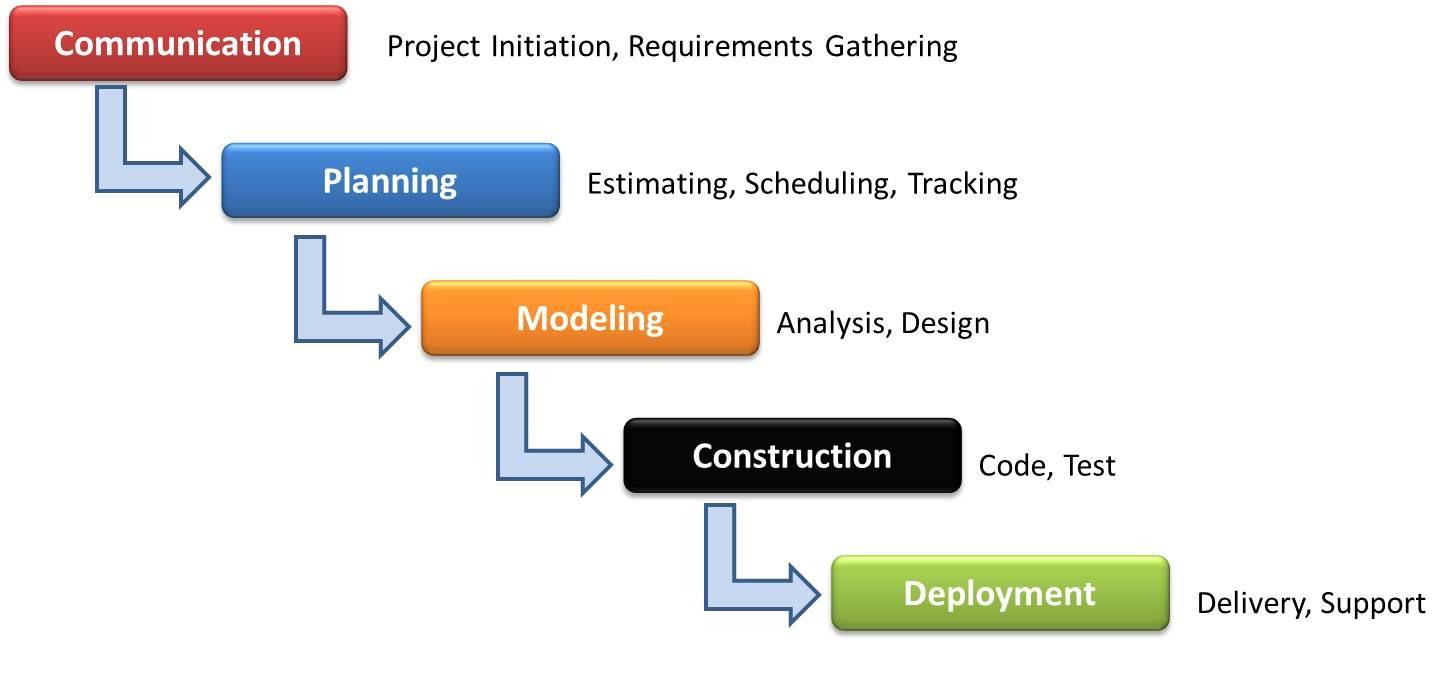
\includegraphics[width=\linewidth]{P3.jpg}
  \caption{Waterfall Model.}
  \label{fig:wmodel}
\end{figure}
\par\noindent The following figures of Task list and Gantt chart shows how the project is controlled and tasks are organized in the team.
\begin{figure}[H] 
  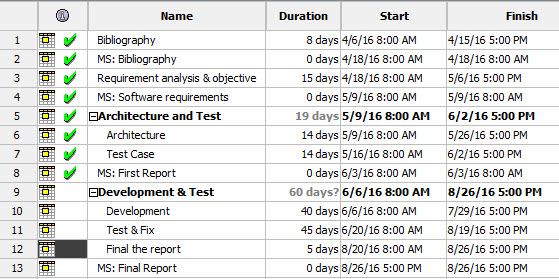
\includegraphics[width=\linewidth]{P1.jpg}
  \caption{Task list.}
  \label{fig:gantt1}
\end{figure}

\par\noindent Mr.Tu and Mr.Quoc are more familiar with the programming language C++ : they are expected to be main developpers of the team. The others Mr.Anh, Ms.Phuong, Mr.Truong are main testers and participate in coding small modules if necessary.
\begin{figure}[H] 
  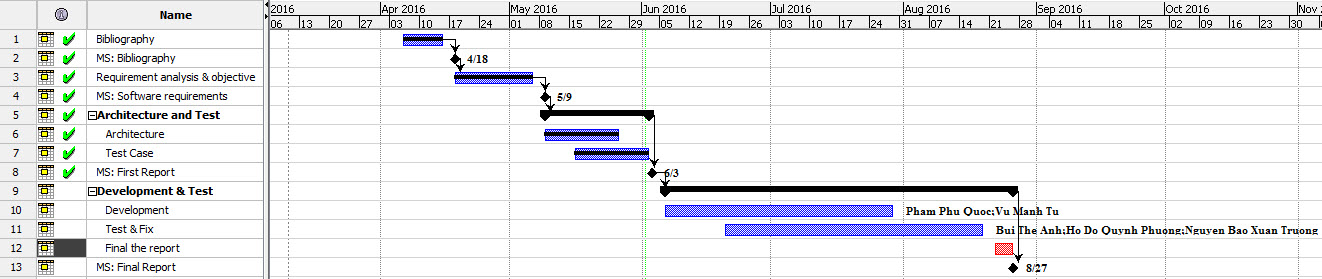
\includegraphics[width=\linewidth]{P2.jpg}
  \caption{Gantt chart.}
  \label{fig:gantt2}
\end{figure} 


\section{Bibliography}
\begin{enumerate}[{(1)}]

\item Digital elevation model. Retrieved from \url{https://en.wikipedia.org/wiki/Digital_elevation_model}. Wikipedia (2016, 9 April).

\item DEM (Digital Elevation Model) files. Retrieved from \url{http://vterrain.org/Elevation/dem.html}.Virtual Terrain Project (n.d.)

\item USGS DEM. Retrieved from \url{https://en.wikipedia.org/wiki/USGS_DEM}. Wikipedia (2016, March 10).

\item Digital Elevation Models - Data User Guide 5. Retrieved from \url{http://agdc.usgs.gov/data/usgs/geodata/dem/dugdem.pdf}. U.S. Geological Survey (1993).

\item Gridded Digital Elevation Model Product Specifications, edition 2.0. Retrieved from \url{http://www.geobc.gov.bc.ca/base-mapping/atlas/trim/specs/BC-DEM-specifications-2002-12.pdf}. Base Mapping and Geomatics Services Branch - Ministry of Sustainable Resource Management - Province of British Columbia (December 2002).

\item Terrain Tools - Importing USGS DEM data Example. Retrieved from \url{http://www.softree.com/Tips_Techniques/T-004-USGS-DEM/USGS_DEM.pdf}. Softree (n.d.).

\item Converting and Using SDTS Digital Elevation Model Data. Retrieved from \url{http://www.esri.com/news/arcuser/0799/webdata6.html}. Mike Price, ESRI (n.d.). 

\item What is SDTS?. Retrieved rom \url{http://mcmcweb.er.usgs.gov/sdts/whatsdts.html}. U.S Geological Survey (n.d.). 

\item 
View the SDTS Document. Retrieved from \url{http://mcmcweb.er.usgs.gov/sdts/standard.html}. U.S. Geological Survey (n.d.).

\item Working with Digital Elevation Models and Digital Terrain Models in Arcmap 9. Retrieved from \url{http://www.lib.uwaterloo.ca/locations/umd/documents/WorkingWithDEM-DTMinArcMap.pdf}. David Findlay (June 2005).

\item DTED. Retrieved from \url{https://en.wikipedia.org/wiki/DTED}. Wikipedia (2016, 31 January).

\item Digital Terrain Elevation Data (DTED) - Part 1. Retrieved from \url{http://www.mission-planning.com/DTED_Part1.htm}. Paul, Pablo's Mission Planning Website (n.d.).

\item Digital Terrain Elevation Data [DTED]. Retrieved from \url{http://fas.org/irp/program/core/dted.htm}. Federation of American Scientists (n.d.).
 
\item Performance specification Digital terrain elevation data (DTED). Retrieved from \url{https://dds.cr.usgs.gov/srtm/version2_1/Documentation/MIL-PDF-89020B.pdf}. U.S. Department of Defense (2000, 23 May).

\item DTED files (Digital Terrain Elevation Data). Retrieved from \url{http://vterrain.org/Elevation/dted.html}. Virtual Terrain Project (n.d.).


\item The DIMAP format. Retrieved from \url{http://www.geo-airbusds.com/en/196-the-dimap-format}. Airbus Defense \& Space (n.d.).

\item Dimap structure. Retrieved from \url{http://www.spotimage.fr/dimap/spec/documentation/3.Dimap_structure.htm}. Airbus Defense \& Space (n.d.).

\item The IDE QtCreator. Retrieved from \url{http://www.qt.io/ide/}. The QtCompany (2016).

\item Richard S., Nicholas H., Graham S. and Benjamin Lipchak. OpenGL Superbible comprehensive tutorial and reference. 5th edition. Addison-Wesley, 2010. Print.
\end{enumerate}

\end{document}
